\section{Design}


\subsection{Kontinuer controller design}
\subsubsection{Systemidentification}

For at kunne estimere dette system, er det første som skulle laves en overføringsfunktion, for den motor samt vippemekanisme som blev brugt til projektet. Her stødte vi på det første problem med systemet, da det ikke var stabilt. Vi blev derfor nød til at indsætte en form for fjedre, for at sikre at systemet var stabilt i en stationær position. Hertil blev der valgt at tilføje en elastik til hver side af bilen, for at opfylde ønsket om et stabilt stationær system. 
Herefter blev målingen lavet for at identificere, en overføringsfunktion for motoren. Da dette system, både skal kunne gå mod højre og venstre, blev der påført et firkantsignal. Herunder i \autoref{fig:system_respons} ses, hvordan responsen \textit{beta} fra motorens tachometer ser ud ved påførelse af firkantsignalet.      


\begin{figure}[H]
	\centering
	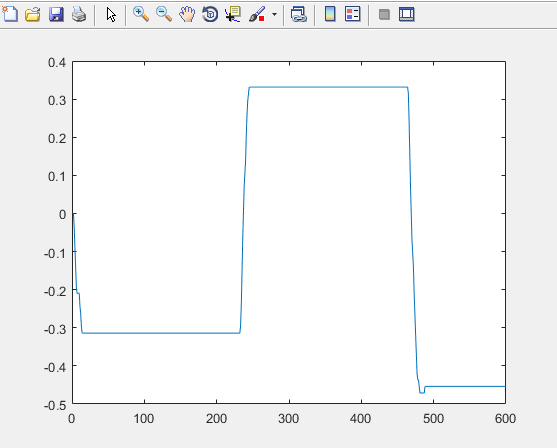
\includegraphics[width = 300pt]{figur/system_respons}
	\caption{System Respons}
	\label{fig:system_respons}
\end{figure}

\begin{lstlisting}[frame=single]
data = iddata(Output,Step,'Ts',Ts);
sys=tfest(data,2,0);%Find overfoeringsfunktion (2p,0z)
\end{lstlisting}

Overføringsfunktionen bliver genereret ud fra funktionen \textit{tfest()}, som estimerer en overføring ud fra inputtet vs outputtet \textit{beta}. Hertil får vi overføringsfunktionen:

\begin{equation}
sys(s) = \frac{188.6}{s^2 + 188.6 s + 358.2}
\end{equation}
    

\subsubsection{Pol placeringskontrol}
For at opfylde vores krav til dynamikken, forsøges der at placeres dominerede poler i systemet. Først findes damping ratio'en ($ \zeta $) ud fra valget om overshoot (OS) på følgende måde: 

\begin{equation}
\zeta = \frac{-\ln(OS/100)}{\sqrt{\pi^2+\ln^2(OS/100)}}
\end{equation} 
Da vi egentlig ikke interesseret i overshoot og har et krav på max 5\% overshoot, så Sættes dampingrationen til 0.9 hvilket svarer til et overshoot på 0.15\% (næsten ingenting)
Dernæst findes båndbredden wn for den karakteristiske ligning ud fra $ \zeta $ og valget om settling time (Ts = 0.5s) på følgede måde:

\begin{equation}
wn = \frac{4}{\zeta*Ts}
\end{equation} 

Til sidst kan den ønskede karakteristiske ligning (Gs) findes og ved:
\begin{equation}
G(s) = \frac{wn^2}{s^2+2*\zeta*wn*s+wn^2}
\end{equation}

Ud fra G(s) isoleres polerne, som skal bruges til at opfylde kravene om settling time (Ts) og overshoot (OS).
\begin{lstlisting}[frame=single]
poles = pole(Gs);
\end{lstlisting}


For vores krav ligger polerne  derfor i -8 \textpm3.8746i. For at fjerne steady state error tilføjes en ekstra pol i 5-10 gange real delen af de dominerende poler. Denne ekstra pol på reel aksen fungere som integrator i kontrolloopet, som korrigerer steady state error'en, men den øger også ordenen af systemet. Polen er valgt 10 gange real delen (5 = minimum for ikke at ændre systemet dynamik betydeligt) af de dominerende poler og bliver derfor -80.


\subsubsection{State space model}

I dette projekt bliver systemets repræsenteret på state space form. Dette gøres for at kunne ændre på state vectorerne, som ændres vha. gainblokke (K), som bliver tilbagekoblet til systemet. For at transformere overføringsfunktion for systemet til en state space model, laves en state space tranformation i matlab. State space formlen giver følgende state space repræsentation

\begin{enumerate}
	
	\item
	$
	A = 
	\begin{bmatrix}
	
	-24.6783 &-358.2121\\
	1.0000      &   0
	\end{bmatrix}
	$
	\item
	$
	B = 
	\begin{bmatrix}
	
	1\\
	0
	\end{bmatrix}
	$    
	
	\item 
	$
	C = 
	\begin{bmatrix}
	
	0  & 188.6101
	\end{bmatrix}
	$    
	\item
	$
	D = 
	\begin{bmatrix}
	
	0  
	\end{bmatrix}
	$  
\end{enumerate}      
Som vist tidligere, er der fundet nogle poler, som ønskes realiseret. Derfor indsættes en K matrix, som skal placeres, i tilbagekoblingen for at opnå de ønskede poler i close-loopet. Først forsøges blot de to konjugerede poler realiseret for at se om kravene til dynamikken er opfyldt, det gøres således:

\begin{lstlisting}[frame=single]
K = place(A,B,poles);

% Define closed loop system
AA = A-B*(K);
sys_CL=ss(AA,B,C,D);
\end{lstlisting}
Her er AA den nye state matrix som står for tilbagekoblingen med K værdierne for at placere de nye poler i Matlab. Resultatet af den tilbagekoblingen kan ses herunder i \autoref{fig:Kontinuer controller 1}. 

\begin{figure}[H]
	\centering
	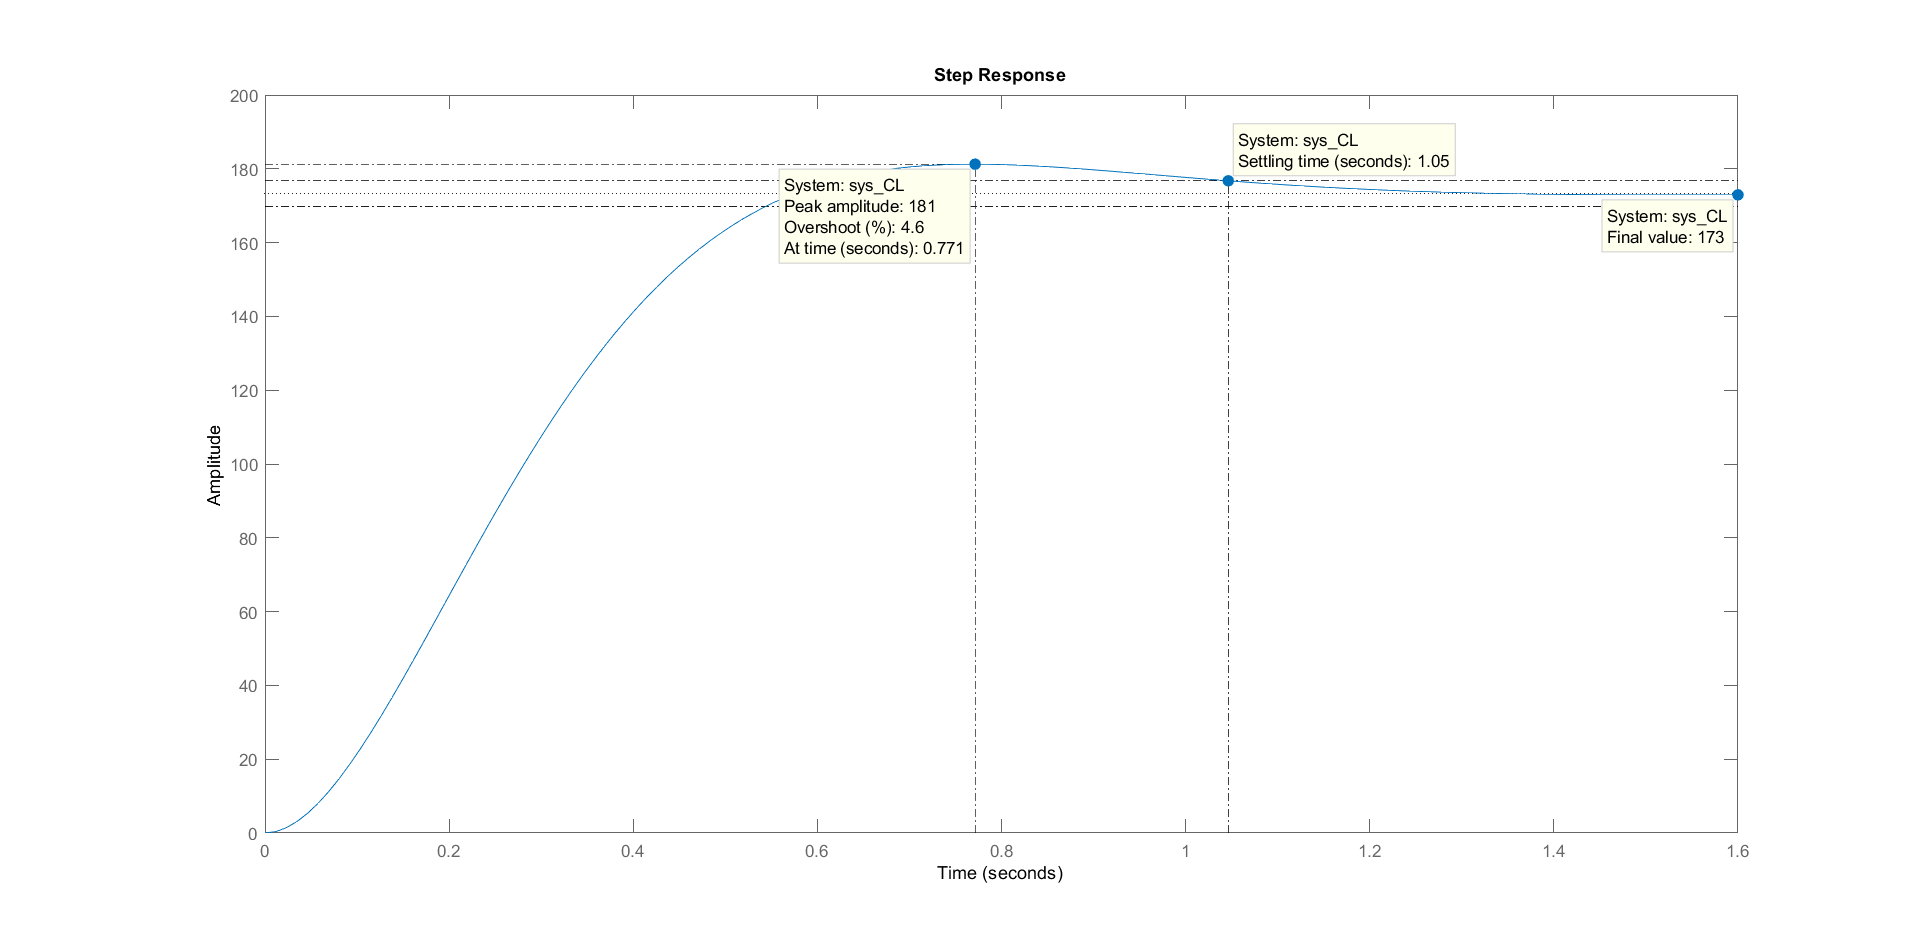
\includegraphics[width = 1\textwidth]{figur/Step_continues_1}
	\caption{Step respons (StepAmplitude = 30) af Kontinuer controller uden steady state error korrektion}
	\label{fig:Kontinuer controller 1}
\end{figure}

Som det kan ses i \autoref{fig:Kontinuer controller 1}, passer dynamikken meget til kravene omkring overhoot og settling time men idet forstærkningen i systemet er for høj, kommer der  betydelig steady state error. Dette kan rettes til ved at tilføje den sidste pol som fjerner fejlen. Men først skal A og B matricen udvides så de kan indeholde den extra state, Dernæst skal alle tre poler placeres igen for at få tre nye K værdier, hvor den sidste er Ke, som ganges på integration polen i loopet. Dette kan ses herunder

\begin{lstlisting}[frame=single]
p3=10*real(poles(1)); % desired location for 3rd pole
pp=[poles; p3];

% Find feedback gains for the desired poles
A_new=[A [0;0];-C 0]; % A matrix after adding an extra state
B_new=[B;0]; % B matrix after adding an extra stat

k = place(A_new,B_new,pp);
K=[k(1) k(2)];
Ke=-k(3);

% Define closed loop system
A_CL=[A-B*K B*Ke;-C 0];
B_CL=[0;0;1];
C_CL=[C 0];
sys_CL=ss(A_CL,B_CL,C_CL,D);
\end{lstlisting}

Her er A\_CL den nye state matrix som står for den udvidet tilbagekoblingen med alle K værdierne for at placere polerne som ønsket i Matlab. Resultatet af den udvidede tilbagekoblingen kan ses herunder i \autoref{fig:Kontinuer controller 2}. 

\begin{figure}[H]
	\centering
	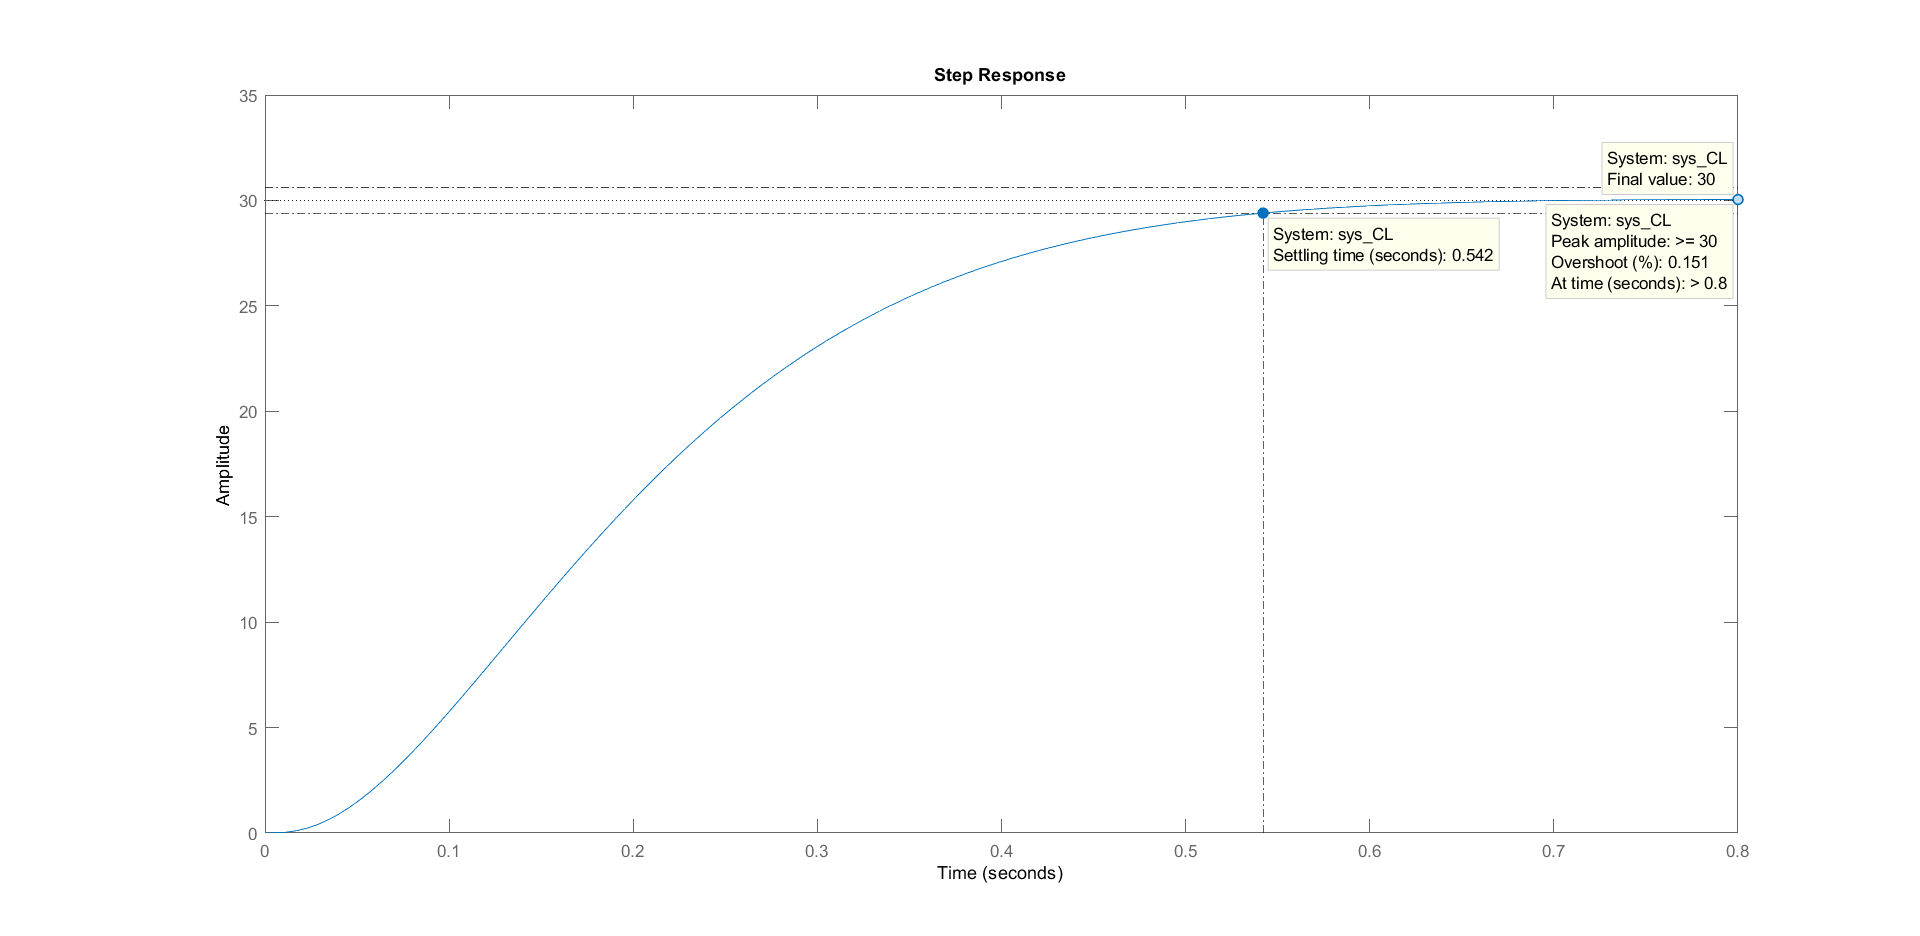
\includegraphics[width = 1\textwidth]{figur/Step_continues_2}
	\caption{Step respons (StepAmplitude = 30) af Kontinuer controller med steady state error korrektion}
	\label{fig:Kontinuer controller 2}
\end{figure}

Som det kan ses i \autoref{fig:Kontinuer controller 2}, passer responsen nu til både kravene omkring overhoot, settling time og steady state error.




\subsubsection{Observer design}
\label{sec:Observer design}
Da systemet i praksis foregår på en LEGO motorblok, kan vi ikke hente states matrixen direkte, da x1 og x2 er en del  af systemet, ift ligningen for state space controller repræsentationen: 
\begin{gather}
\dot{x}=Ax+Bu \\
y=Cx
\end{gather}
Derfor indsættes yderligere en blok i systemet, for at kunne observere ind og output, og på baggrund af dem, og den beregnede state matrix, beregnes en estimeret xhat, som skal bruges til tilbagekoblingen, som erstatning for states matrixen \\
Observer ligningen hedder:


\begin{gather}
\dot{\hat{x}}=A\hat{x}+Bu+L(y-\hat{y}) \\
\hat{y}=C\hat{x}
\end{gather}


Det er den formel vi bruger til at lave vores observer.\\

Først skal vi vælge observatørens forstærkningsmatrice $ L $. Da vi ønsker at observerens dynamik skal være meget hurtigere end selve systemet, skal vi placere polerne mindst fem gange længere til venstre end systemets dominerende poler. Vi kan designe observerens forstærkning med følgende kommando uden at transformere vores state space respræsentation til observer canonical form

\begin{lstlisting}[frame=single]
%Valg af poler er polerne ganget med 5
poles_L = poles*5; 
%Beregning af L
L = place(A', C', poles_L)'; 
\end{lstlisting}

Derfor kan observatøren nu implementeres i Simulink og bruges til at hente et gæt på state matricen ud fra outputtet y (rho) fra gyroskopet og inputtet u til motor blokken. Denne implementering følger observer ligningen fra før og kan ses i diagrammet herunder i \autoref{fig:Simulink_observer_continues}

\begin{figure}[H]
	\centering
	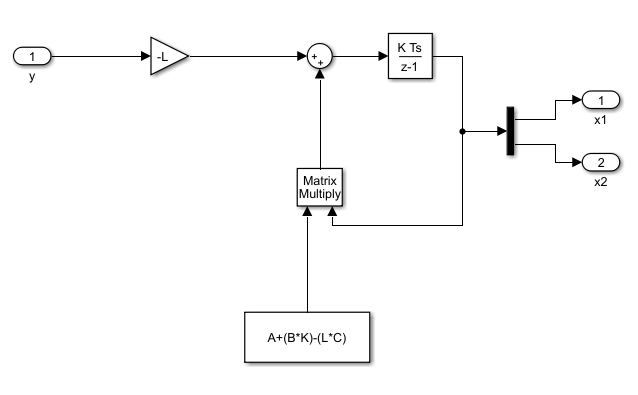
\includegraphics[width = 1\textwidth]{figur/Simulink_observer_continues}
	\caption{Kontinuer observer}
	\label{fig:Simulink_observer_continues}
\end{figure}


\subsection{Diskret controller design}
\subsubsection{Systemidentification}
For at kunne implementere systemet på en microcontroller - som på LEGO EV3, kan systemet med fordel transformeres til en diskret state space model. Dette kommer af at reguleringen skal foregå på et digitalt system, som sampler med en bestemt frekvens. Både overføringsfunktionen og state space repræsentationen bliver transformeret til diskrete værdier, det samme gøres ved vores poler, hvormed K værdierne ændres til de passende værdier. Alt dette gøres igennem matlab, hvor funktionen c2d() bliver brugt. Fremgangs måden  er ellers den samme som ved den Kontinuer controller. 

\begin{lstlisting}[frame=single]
Ts = 0.01;
sysD=c2d(sys,Ts,'zoh'); %samplingstiden er 0.01s
\end{lstlisting}

Først overføres den kontinuere overføringsfunktion fra før til det diskrete domæne ved hjælp af c2d() med samplingstiden 0.01s og "zoh" metoden til følgende resultat:

\begin{equation}
sysD(z) = \frac{0.008675 z^{-1} + + 0.007989 z^{-2}}{1 - 1.75 z^{-1} + 0.7813 z^{-2}}
\end{equation}

\subsubsection{Pol placeringskontrol}
Idet den karakteristiske ligning (Gs) som bestemmer systemet dynamik allerede er bestemt i det kontinuere domæne  transformeres denne og så til det diskrete domæne G(z) med c2d() med samplingstiden 0.01s og denne gang "tustin" metoden for at få så præcist match i frekvensdomænet mellem den kontinuere og diskrete model af karakteristiske ligning. 

\begin{lstlisting}[frame=single]
Gz = c2d(Gs,Ts,'tustin');
poles_z = pole(Gz);
\end{lstlisting}

Ud fra G(z) isoleres polerne, som skal bruges til at opfylde kravene om settling time (Ts) og overshoot (OS). For vores krav ligger polerne  derfor i 0.9224 \textpm0.0358i, som begge ligger inden for enheds cirklen og derfor er stabile.  
Desværre stødte vi ind i problemer med at fjerne steady state error i det diskrete domæne, men det burde kunne fjerned ved at z-transformere den pol som ligger i -80 fra den kontinuere model til z-domænet. Dette problem er dog ikke blevet løst og derfor ses der bort fra steady state error i den diskrete model.

\subsubsection{State space model}

 For igen at kunne ændre på state vectorerne i den diskete model, som også ændres vha. gainblokke (Kd) tilbagekoblet til systemet, så skal den diskrete overføringsfunktio transformeres til en state space model. State space formlen giver følgende state space repræsentation for den  diskrete model.

\begin{enumerate}
	
	\item
	$
	Ad = 
	\begin{bmatrix}
	
	1.7497  & -0.7813\\
	1.0000   &      0
	\end{bmatrix}
	$
	\item
	$
	Bd = 
	\begin{bmatrix}
	
	1\\
	0
	\end{bmatrix}
	$    
	
	\item 
	$
	Cd = 
	\begin{bmatrix}
	
	0.0087  &  0.0080
	\end{bmatrix}
	$    
	\item
	$
	Dd = 
	\begin{bmatrix}
	
	0  
	\end{bmatrix}
	$  
\end{enumerate}      
Polerne, som ønskes realiseret, virkeliggøre ved indsættes en Kd matrix, som skal placeres, i tilbagekoblingen for at opnå de ønskede poler i close-loopet. Her forsøges blot de to konjugerede poler realiseret for at se om kravene til dynamikken er opfyldt, det gøres således:

\begin{lstlisting}[frame=single]
Kd = place(Ad,Bd,poles_z);

% Define closed loop system
AAd = Ad-Bd*(Kd);
sysD_CL=ss(AAd,Bd,Cd,Dd,Ts);
\end{lstlisting}
Her er AAd den nye state matrix som står for tilbagekoblingen med Kd værdierne for at placere de nye poler i Matlab. Resultatet af den tilbagekoblingen kan ses herunder i \autoref{fig:Diskret controller 1}. 

\begin{figure}[H]
	\centering
	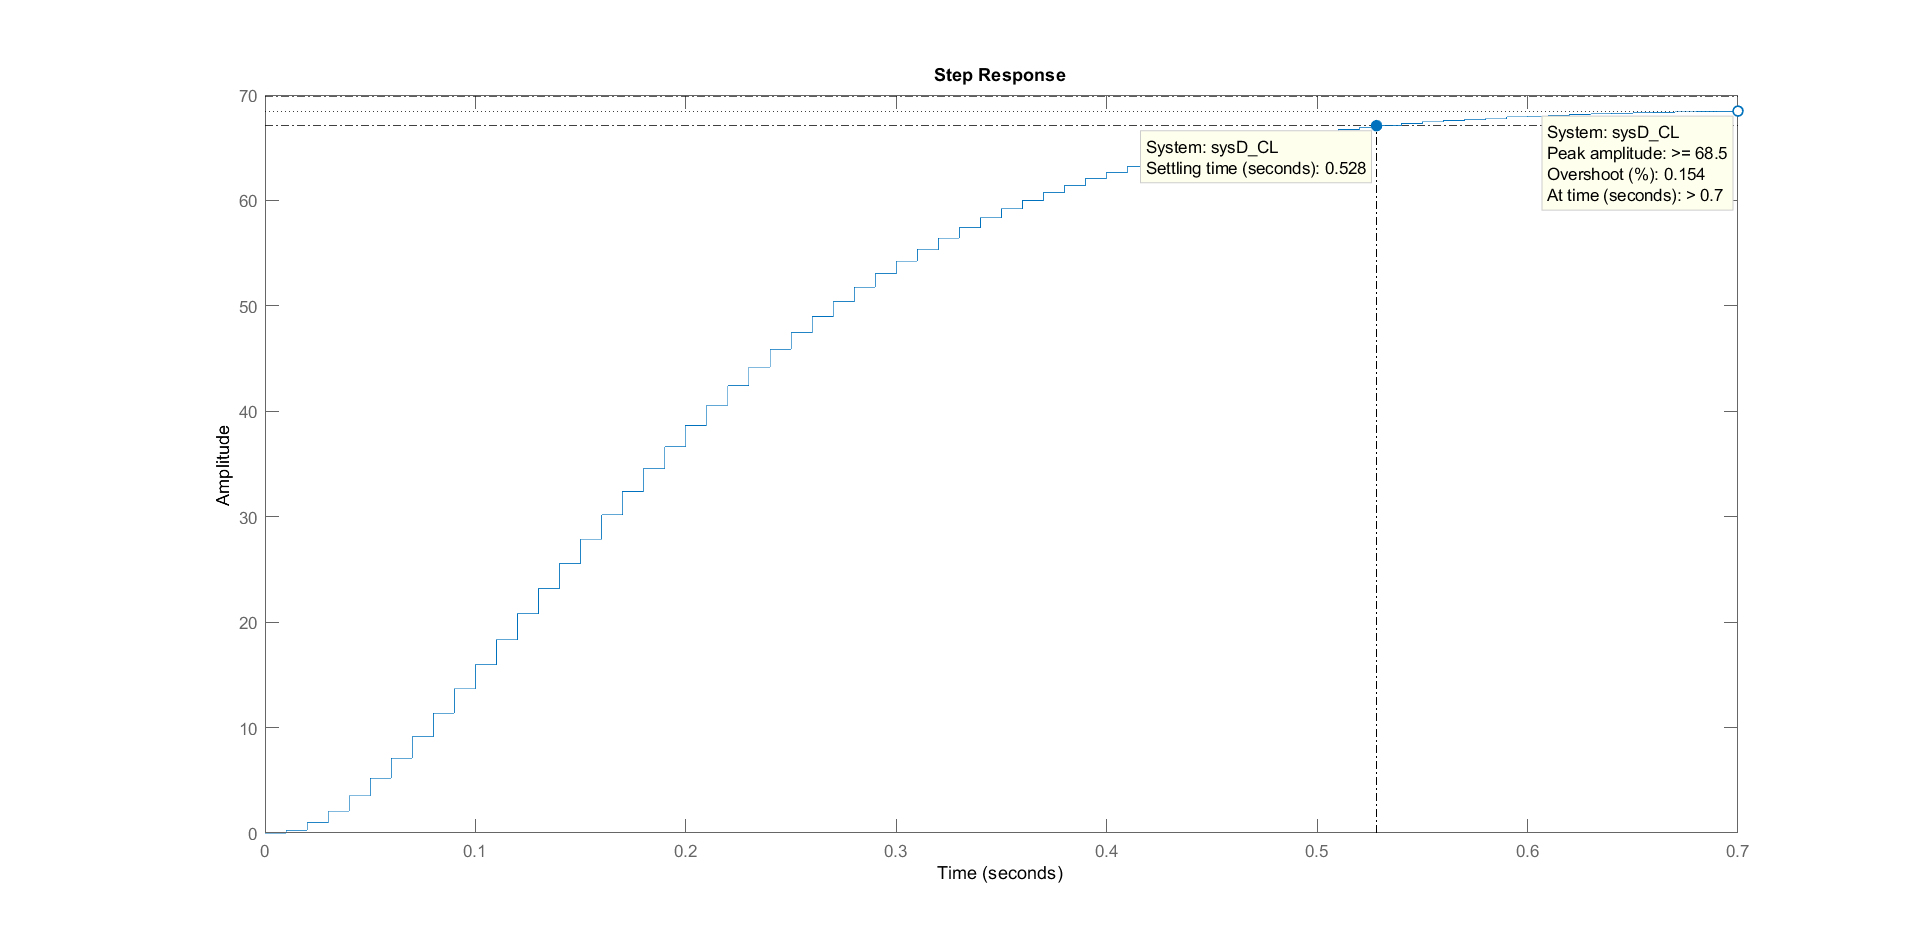
\includegraphics[width = 1\textwidth]{figur/Step_diskret_1}
	\caption{Step respons (StepAmplitude = 30) af diskret controller uden steady state error korrektion}
	\label{fig:Diskret controller 1}
\end{figure}




Som det kan ses i \autoref{fig:Diskret controller 1}, passer dynamikken meget til kravene omkring overhoot og settling time. Forstærkningen i systemet er dog for høj hvilket resulterer i betydelig steady state error. Dette kan rettes til som nævnt tidligere ved at tilføje den sidste pol som fjerner fejlen. Dette er dog ikke gjort ved den diskrete controller model. 

\subsubsection{Observer design}
Observer delen er den samme som i den kontinuere controller model og følger observer ligningen:
\begin{gather}
\dot{\hat{x}}=Ad\hat{x}+Bdu+Ld(y-\hat{y}) \\
\hat{y}=Cd\hat{x}
\end{gather}

Først skal vi vælge observatørens forstærkningsmatrice $ Ld $. Da vi allerede har fundet observerens dynamik og tilhørende poler i den kontinuere controller så kan vi blot transformere disse poler til det diskrete domæne med c2d(). Vi kan designe observerens forstærkning med følgende kommando uden at transformere vores state space respræsentation til observer canonical form
\begin{lstlisting}[frame=single]
%valg af Ld poler 
GLs = (1/(s-poles_L(1)))*(1/(s-poles_L(2)));
GLz = c2d(GLs,Ts,'tustin');
poles_Ld =pole(GLz);
%beregning af Ld
Ld = place(Ad', Cd', poles_Ld)';  
\end{lstlisting}

Derfor kan observatøren nu implementeres i Simulink og bruges til at hente et gæt på state matricen ud fra outputtet y (rho) fra gyroskopet og inputtet u til motor blokken. Denne implementering følger observer ligningen fra før og kan ses i diagrammet herunder i \autoref{fig:Simulink_observer_diskret}
Den eneste ændring i forhold til den kontinuere observer er at integration blokken nu er udskiftets med en unit delay blok for at realisere den samplede state matrix   

\begin{figure}[H]
	\centering
	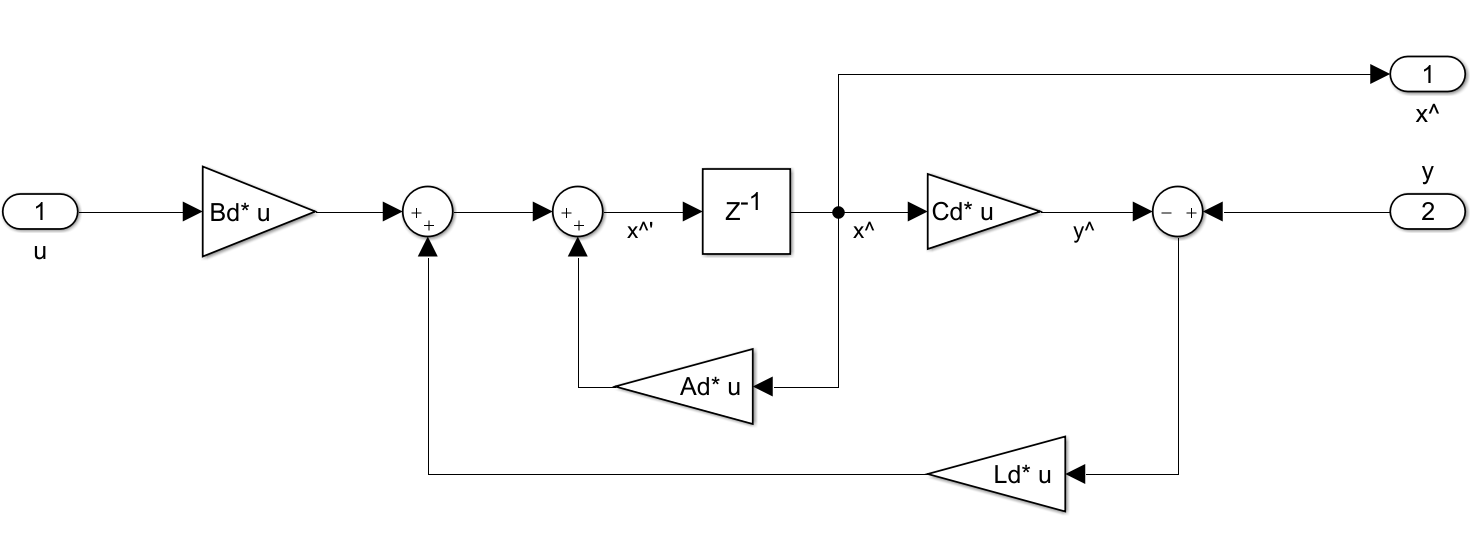
\includegraphics[width = 1\textwidth]{figur/Simulink_observer_diskret}
	\caption{Diskret observer}
	\label{fig:Simulink_observer_diskret}
\end{figure}


